\documentclass[12pt]{article}
\usepackage[english]{babel}
\usepackage[utf8]{inputenc}
\usepackage{amsmath, amssymb, amsthm}
\usepackage{graphicx}
\usepackage{hyperref}
\usepackage[margin=.75in]{geometry}
\usepackage{xcolor}
\usepackage{tikz}
\usepackage{gensymb}

\newtheorem{theorem}{Theorem}
\newtheorem{prop}{Proposition}
\newtheorem*{prop*}{Proposition}
\newtheorem{obs}{Observation}
\newtheorem*{obs*}{Observation}

\setlength{\topmargin}{0pt}
\setlength{\headsep}{0pt}
\textheight = 600pt

\title{Graph Theory \\ Homework 8}
\author{Ben Kallus and Nicholas Adair}
\date{Due Monday, Monday, March 15}

\begin{document}
\maketitle

\noindent{\bf 4.25}

    The following are all of the spanning trees for $G$:
    \begin{center}
        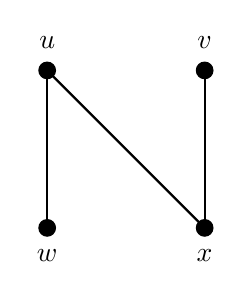
\begin{tikzpicture}
            \draw[fill=black] (0.0, 2.0) circle (3pt);
            \node at (0.0, 2.35) {$u$};
            \draw[fill=black] (0.0, 0.0) circle (3pt);
            \node at (0.0, -0.35) {$w$};
            \draw[fill=black] (2.0, 0.0) circle (3pt);
            \node at (2.0, -0.35) {$x$};
            \draw[fill=black] (2.0, 2.0) circle (3pt);
            \node at (2.0, 2.35) {$v$};

            \draw[thick] (0.0, 2.0) -- (0.0, 0.0); % u-w
            \draw[thick] (0.0, 2.0) -- (2.0, 0.0); % u-x
            \draw[thick] (2.0, 2.0) -- (2.0, 0.0); % v-x
        \end{tikzpicture}
        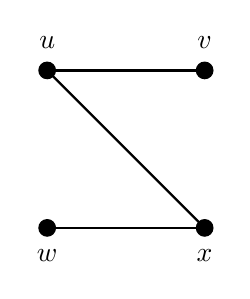
\begin{tikzpicture}
            \draw[fill=black] (0.0, 2.0) circle (3pt);
            \node at (0.0, 2.35) {$u$};
            \draw[fill=black] (0.0, 0.0) circle (3pt);
            \node at (0.0, -0.35) {$w$};
            \draw[fill=black] (2.0, 0.0) circle (3pt);
            \node at (2.0, -0.35) {$x$};
            \draw[fill=black] (2.0, 2.0) circle (3pt);
            \node at (2.0, 2.35) {$v$};

            \draw[thick] (0.0, 2.0) -- (2.0, 0.0); % u-x
            \draw[thick] (0.0, 2.0) -- (2.0, 2.0); % u-v
            \draw[thick] (0.0, 0.0) -- (2.0, 0.0); % w-x
        \end{tikzpicture}
        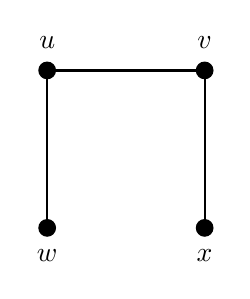
\begin{tikzpicture}
            \draw[fill=black] (0.0, 2.0) circle (3pt);
            \node at (0.0, 2.35) {$u$};
            \draw[fill=black] (0.0, 0.0) circle (3pt);
            \node at (0.0, -0.35) {$w$};
            \draw[fill=black] (2.0, 0.0) circle (3pt);
            \node at (2.0, -0.35) {$x$};
            \draw[fill=black] (2.0, 2.0) circle (3pt);
            \node at (2.0, 2.35) {$v$};

            \draw[thick] (0.0, 2.0) -- (0.0, 0.0); % u-w
            \draw[thick] (0.0, 2.0) -- (2.0, 2.0); % u-v
            \draw[thick] (2.0, 2.0) -- (2.0, 0.0); % v-x
        \end{tikzpicture}
        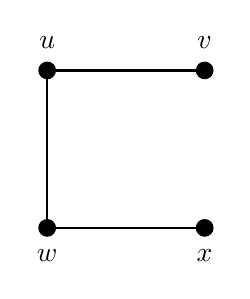
\begin{tikzpicture}
            \draw[fill=black] (0.0, 2.0) circle (3pt);
            \node at (0.0, 2.35) {$u$};
            \draw[fill=black] (0.0, 0.0) circle (3pt);
            \node at (0.0, -0.35) {$w$};
            \draw[fill=black] (2.0, 0.0) circle (3pt);
            \node at (2.0, -0.35) {$x$};
            \draw[fill=black] (2.0, 2.0) circle (3pt);
            \node at (2.0, 2.35) {$v$};

            \draw[thick] (0.0, 2.0) -- (0.0, 0.0); % u-w
            \draw[thick] (0.0, 2.0) -- (2.0, 2.0); % u-v
            \draw[thick] (0.0, 0.0) -- (2.0, 0.0); % w-x
        \end{tikzpicture}
        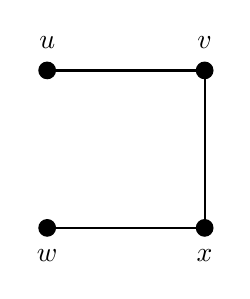
\begin{tikzpicture}
            \draw[fill=black] (0.0, 2.0) circle (3pt);
            \node at (0.0, 2.35) {$u$};
            \draw[fill=black] (0.0, 0.0) circle (3pt);
            \node at (0.0, -0.35) {$w$};
            \draw[fill=black] (2.0, 0.0) circle (3pt);
            \node at (2.0, -0.35) {$x$};
            \draw[fill=black] (2.0, 2.0) circle (3pt);
            \node at (2.0, 2.35) {$v$};

            \draw[thick] (0.0, 2.0) -- (2.0, 2.0); % u-v
            \draw[thick] (0.0, 0.0) -- (2.0, 0.0); % w-x
            \draw[thick] (2.0, 2.0) -- (2.0, 0.0); % v-x
        \end{tikzpicture}
        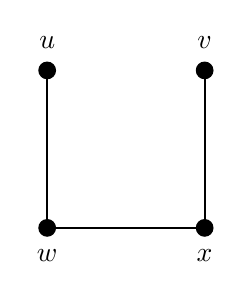
\begin{tikzpicture}
            \draw[fill=black] (0.0, 2.0) circle (3pt);
            \node at (0.0, 2.35) {$u$};
            \draw[fill=black] (0.0, 0.0) circle (3pt);
            \node at (0.0, -0.35) {$w$};
            \draw[fill=black] (2.0, 0.0) circle (3pt);
            \node at (2.0, -0.35) {$x$};
            \draw[fill=black] (2.0, 2.0) circle (3pt);
            \node at (2.0, 2.35) {$v$};

            \draw[thick] (0.0, 2.0) -- (0.0, 0.0); % u-w
            \draw[thick] (0.0, 0.0) -- (2.0, 0.0); % w-x
            \draw[thick] (2.0, 2.0) -- (2.0, 0.0); % v-x
        \end{tikzpicture}

        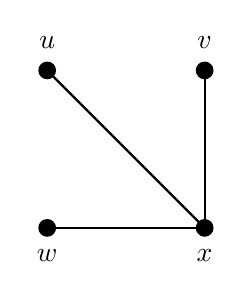
\begin{tikzpicture}
            \draw[fill=black] (0.0, 2.0) circle (3pt);
            \node at (0.0, 2.35) {$u$};
            \draw[fill=black] (0.0, 0.0) circle (3pt);
            \node at (0.0, -0.35) {$w$};
            \draw[fill=black] (2.0, 0.0) circle (3pt);
            \node at (2.0, -0.35) {$x$};
            \draw[fill=black] (2.0, 2.0) circle (3pt);
            \node at (2.0, 2.35) {$v$};

            \draw[thick] (0.0, 2.0) -- (2.0, 0.0); % u-x
            \draw[thick] (0.0, 0.0) -- (2.0, 0.0); % w-x
            \draw[thick] (2.0, 2.0) -- (2.0, 0.0); % v-x
        \end{tikzpicture}
        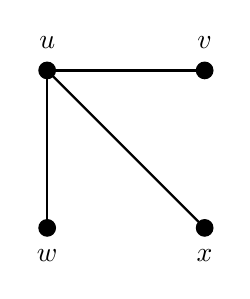
\begin{tikzpicture}
            \draw[fill=black] (0.0, 2.0) circle (3pt);
            \node at (0.0, 2.35) {$u$};
            \draw[fill=black] (0.0, 0.0) circle (3pt);
            \node at (0.0, -0.35) {$w$};
            \draw[fill=black] (2.0, 0.0) circle (3pt);
            \node at (2.0, -0.35) {$x$};
            \draw[fill=black] (2.0, 2.0) circle (3pt);
            \node at (2.0, 2.35) {$v$};

            \draw[thick] (0.0, 2.0) -- (0.0, 0.0); % u-w
            \draw[thick] (0.0, 2.0) -- (2.0, 0.0); % u-x
            \draw[thick] (0.0, 2.0) -- (2.0, 2.0); % u-v
        \end{tikzpicture}
    \end{center}

    The first row of spanning trees are all isomorphic, since they are all $P_3$.
    The second row of spanning trees are isomorphic, since the graph on the left can be obtained from the graph on the right through a $180\degree$ rotation.

    We can be certain that these are all possible spanning trees for $G$.
    Since $G$ is of order 4, a spanning tree for $G$ must have 3 edges.
    Since $G$ is of size 5, each spanning tree of $G$ can be obtained from $G$ by removing 2 edges from $G$.
    Thus, there are at most ${5 \choose 2} = 10$ spanning trees for $G$.
    Since removing $uv,uw$ or $xv,xw$ would disconnect the graph, there are at most 8 spanning trees for $G$.
    Thus, we have found all spanning trees for $G$.

    \newpage
    The following are all of the spanning trees for $H$:
    \begin{center}
        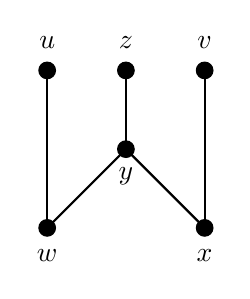
\begin{tikzpicture}
            \draw[fill=black] (0.0, 0.0) circle (3pt);
            \node at (0.0, -0.35) {$w$};
            \draw[fill=black] (1.0, 1.0) circle (3pt);
            \node at (1.0, .65) {$y$};
            \draw[fill=black] (2.0, 0.0) circle (3pt);
            \node at (2.0, -0.35) {$x$};
            \draw[fill=black] (2.0, 2.0) circle (3pt);
            \node at (2.0, 2.35) {$v$};
            \draw[fill=black] (0.0, 2.0) circle (3pt);
            \node at (0.0, 2.35) {$u$};
            \draw[fill=black] (1.0, 2.0) circle (3pt);
            \node at (1.0, 2.35) {$z$};

            \draw[thick] (0.0, 2.0) -- (0.0, 0.0); % u-w
            \draw[thick] (0.0, 0.0) -- (1.0, 1.0); % w-y
            \draw[thick] (2.0, 0.0) -- (1.0, 1.0); % y-x
            \draw[thick] (2.0, 2.0) -- (2.0, 0.0); % v-x
            \draw[thick] (1.0, 1.0) -- (1.0, 2.0); % y-z
        \end{tikzpicture}
        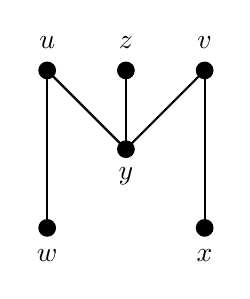
\begin{tikzpicture}
            \draw[fill=black] (0.0, 0.0) circle (3pt);
            \node at (0.0, -0.35) {$w$};
            \draw[fill=black] (1.0, 1.0) circle (3pt);
            \node at (1.0, .65) {$y$};
            \draw[fill=black] (2.0, 0.0) circle (3pt);
            \node at (2.0, -0.35) {$x$};
            \draw[fill=black] (2.0, 2.0) circle (3pt);
            \node at (2.0, 2.35) {$v$};
            \draw[fill=black] (0.0, 2.0) circle (3pt);
            \node at (0.0, 2.35) {$u$};
            \draw[fill=black] (1.0, 2.0) circle (3pt);
            \node at (1.0, 2.35) {$z$};

            \draw[thick] (0.0, 2.0) -- (0.0, 0.0); % u-w
            \draw[thick] (1.0, 1.0) -- (0.0, 2.0); % u-y
            \draw[thick] (1.0, 1.0) -- (2.0, 2.0); % y-v
            \draw[thick] (2.0, 2.0) -- (2.0, 0.0); % v-x
            \draw[thick] (1.0, 1.0) -- (1.0, 2.0); % y-z
        \end{tikzpicture}
        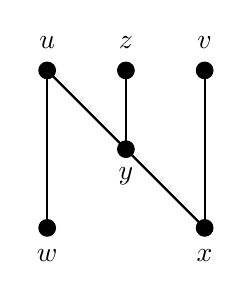
\begin{tikzpicture}
            \draw[fill=black] (0.0, 0.0) circle (3pt);
            \node at (0.0, -0.35) {$w$};
            \draw[fill=black] (1.0, 1.0) circle (3pt);
            \node at (1.0, .65) {$y$};
            \draw[fill=black] (2.0, 0.0) circle (3pt);
            \node at (2.0, -0.35) {$x$};
            \draw[fill=black] (2.0, 2.0) circle (3pt);
            \node at (2.0, 2.35) {$v$};
            \draw[fill=black] (0.0, 2.0) circle (3pt);
            \node at (0.0, 2.35) {$u$};
            \draw[fill=black] (1.0, 2.0) circle (3pt);
            \node at (1.0, 2.35) {$z$};

            \draw[thick] (0.0, 2.0) -- (0.0, 0.0); % u-w
            \draw[thick] (1.0, 1.0) -- (0.0, 2.0); % u-y
            \draw[thick] (2.0, 0.0) -- (1.0, 1.0); % y-x
            \draw[thick] (2.0, 2.0) -- (2.0, 0.0); % v-x
            \draw[thick] (1.0, 1.0) -- (1.0, 2.0); % y-z
        \end{tikzpicture}
        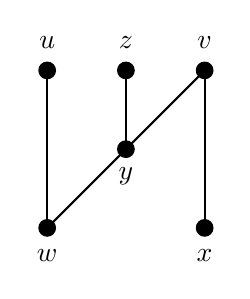
\begin{tikzpicture}
            \draw[fill=black] (0.0, 0.0) circle (3pt);
            \node at (0.0, -0.35) {$w$};
            \draw[fill=black] (1.0, 1.0) circle (3pt);
            \node at (1.0, .65) {$y$};
            \draw[fill=black] (2.0, 0.0) circle (3pt);
            \node at (2.0, -0.35) {$x$};
            \draw[fill=black] (2.0, 2.0) circle (3pt);
            \node at (2.0, 2.35) {$v$};
            \draw[fill=black] (0.0, 2.0) circle (3pt);
            \node at (0.0, 2.35) {$u$};
            \draw[fill=black] (1.0, 2.0) circle (3pt);
            \node at (1.0, 2.35) {$z$};

            \draw[thick] (0.0, 2.0) -- (0.0, 0.0); % u-w
            \draw[thick] (0.0, 0.0) -- (1.0, 1.0); % w-y
            \draw[thick] (1.0, 1.0) -- (2.0, 2.0); % y-v
            \draw[thick] (2.0, 2.0) -- (2.0, 0.0); % v-x
            \draw[thick] (1.0, 1.0) -- (1.0, 2.0); % y-z
        \end{tikzpicture}

        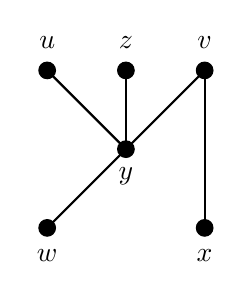
\begin{tikzpicture}
            \draw[fill=black] (0.0, 0.0) circle (3pt);
            \node at (0.0, -0.35) {$w$};
            \draw[fill=black] (1.0, 1.0) circle (3pt);
            \node at (1.0, .65) {$y$};
            \draw[fill=black] (2.0, 0.0) circle (3pt);
            \node at (2.0, -0.35) {$x$};
            \draw[fill=black] (2.0, 2.0) circle (3pt);
            \node at (2.0, 2.35) {$v$};
            \draw[fill=black] (0.0, 2.0) circle (3pt);
            \node at (0.0, 2.35) {$u$};
            \draw[fill=black] (1.0, 2.0) circle (3pt);
            \node at (1.0, 2.35) {$z$};

            \draw[thick] (0.0, 0.0) -- (1.0, 1.0); % w-y
            \draw[thick] (1.0, 1.0) -- (0.0, 2.0); % u-y
            \draw[thick] (1.0, 1.0) -- (2.0, 2.0); % y-v
            \draw[thick] (2.0, 2.0) -- (2.0, 0.0); % v-x
            \draw[thick] (1.0, 1.0) -- (1.0, 2.0); % y-z
        \end{tikzpicture}
        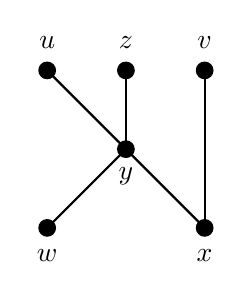
\begin{tikzpicture}
            \draw[fill=black] (0.0, 0.0) circle (3pt);
            \node at (0.0, -0.35) {$w$};
            \draw[fill=black] (1.0, 1.0) circle (3pt);
            \node at (1.0, .65) {$y$};
            \draw[fill=black] (2.0, 0.0) circle (3pt);
            \node at (2.0, -0.35) {$x$};
            \draw[fill=black] (2.0, 2.0) circle (3pt);
            \node at (2.0, 2.35) {$v$};
            \draw[fill=black] (0.0, 2.0) circle (3pt);
            \node at (0.0, 2.35) {$u$};
            \draw[fill=black] (1.0, 2.0) circle (3pt);
            \node at (1.0, 2.35) {$z$};

            \draw[thick] (0.0, 0.0) -- (1.0, 1.0); % w-y
            \draw[thick] (1.0, 1.0) -- (0.0, 2.0); % u-y
            \draw[thick] (2.0, 0.0) -- (1.0, 1.0); % y-x
            \draw[thick] (2.0, 2.0) -- (2.0, 0.0); % v-x
            \draw[thick] (1.0, 1.0) -- (1.0, 2.0); % y-z
        \end{tikzpicture}
        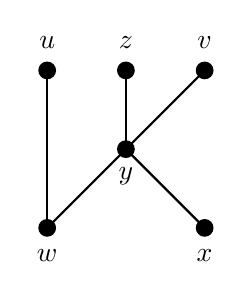
\begin{tikzpicture}
            \draw[fill=black] (0.0, 0.0) circle (3pt);
            \node at (0.0, -0.35) {$w$};
            \draw[fill=black] (1.0, 1.0) circle (3pt);
            \node at (1.0, .65) {$y$};
            \draw[fill=black] (2.0, 0.0) circle (3pt);
            \node at (2.0, -0.35) {$x$};
            \draw[fill=black] (2.0, 2.0) circle (3pt);
            \node at (2.0, 2.35) {$v$};
            \draw[fill=black] (0.0, 2.0) circle (3pt);
            \node at (0.0, 2.35) {$u$};
            \draw[fill=black] (1.0, 2.0) circle (3pt);
            \node at (1.0, 2.35) {$z$};

            \draw[thick] (0.0, 2.0) -- (0.0, 0.0); % u-w
            \draw[thick] (0.0, 0.0) -- (1.0, 1.0); % w-y
            \draw[thick] (2.0, 0.0) -- (1.0, 1.0); % y-x
            \draw[thick] (1.0, 1.0) -- (2.0, 2.0); % y-v
            \draw[thick] (1.0, 1.0) -- (1.0, 2.0); % y-z
        \end{tikzpicture}
        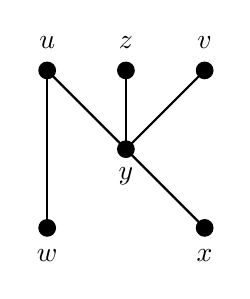
\begin{tikzpicture}
            \draw[fill=black] (0.0, 0.0) circle (3pt);
            \node at (0.0, -0.35) {$w$};
            \draw[fill=black] (1.0, 1.0) circle (3pt);
            \node at (1.0, .65) {$y$};
            \draw[fill=black] (2.0, 0.0) circle (3pt);
            \node at (2.0, -0.35) {$x$};
            \draw[fill=black] (2.0, 2.0) circle (3pt);
            \node at (2.0, 2.35) {$v$};
            \draw[fill=black] (0.0, 2.0) circle (3pt);
            \node at (0.0, 2.35) {$u$};
            \draw[fill=black] (1.0, 2.0) circle (3pt);
            \node at (1.0, 2.35) {$z$};

            \draw[thick] (0.0, 2.0) -- (0.0, 0.0); % u-w
            \draw[thick] (1.0, 1.0) -- (0.0, 2.0); % u-y
            \draw[thick] (2.0, 0.0) -- (1.0, 1.0); % y-x
            \draw[thick] (1.0, 1.0) -- (2.0, 2.0); % y-v
            \draw[thick] (1.0, 1.0) -- (1.0, 2.0); % y-z
        \end{tikzpicture}

        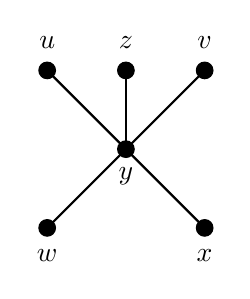
\begin{tikzpicture}
            \draw[fill=black] (0.0, 0.0) circle (3pt);
            \node at (0.0, -0.35) {$w$};
            \draw[fill=black] (1.0, 1.0) circle (3pt);
            \node at (1.0, .65) {$y$};
            \draw[fill=black] (2.0, 0.0) circle (3pt);
            \node at (2.0, -0.35) {$x$};
            \draw[fill=black] (2.0, 2.0) circle (3pt);
            \node at (2.0, 2.35) {$v$};
            \draw[fill=black] (0.0, 2.0) circle (3pt);
            \node at (0.0, 2.35) {$u$};
            \draw[fill=black] (1.0, 2.0) circle (3pt);
            \node at (1.0, 2.35) {$z$};

            \draw[thick] (0.0, 0.0) -- (1.0, 1.0); % w-y
            \draw[thick] (1.0, 1.0) -- (0.0, 2.0); % u-y
            \draw[thick] (2.0, 0.0) -- (1.0, 1.0); % y-x
            \draw[thick] (1.0, 1.0) -- (2.0, 2.0); % y-v
            \draw[thick] (1.0, 1.0) -- (1.0, 2.0); % y-z
        \end{tikzpicture}
    \end{center}

    The graphs in the first row of spanning trees are all isomorphic, since they can be transformed into each other by swapping the locations of their left and right ``legs."
    The graphs in the second row of spanning trees are all isomorphic because the first two are mirrors of the last two, and the first can be transformed into the second by swapping the locations of $v$ and $x$.

    We can be certain that these are all possible spanning trees for $H$. Since $H$ is of order 6, a spanning tree for $H$ must have 5 edges.
    Since $H$ is of size 7, each spanning tree of $H$ can be obtained from $H$ by removing 2 edges from $H$.
    Since $yz$ is a bridge, it must be present in any spanning tree of $H$.
    Since removing any two of $\{uy, wy, uw\}$ would disconnect the graph, at least two of the edges in that set must be present in any spanning tree of $H$.
    Similarly, at least two of $\{vy, xy, vx\}$ must be present in any spanning tree of $H$.
    Thus, each spanning tree of $H$ can be expressed as $H - e_1 - e_2$ for some $e_1 \in \{uy, wy, uw\}$, and some $e_2 \in \{vy, xy, vx\}$.
    Thus, there are ${3 \choose 1} \cdot {3 \choose 1} = 9$ spanning trees of $H$.

\newpage\noindent{\bf 4.26} Proposition: An edge $e$ of a connected graph $G$ is a bridge if and only if $e$ belongs to every spanning tree of $G$.
\begin{proof}
    Let $G$ be a connected graph.
    Let $e \in E(G)$.

    Suppose that $e$ is a bridge.
    Then, $G-e$ is disconnected.
    Thus, every spanning subgraph of $G-e$ is disconnected, so every spanning tree of $G$ must include $e$.

    Now, suppose that every spanning tree of $G$ contains $e$.
    Assume, toward a contradiction, that $e$ is not a bridge.
    Then, $G-e$ is connected.
    Let $T$ be a spanning tree of $G-e$.
    Then, $e \notin E(T)$.
    Since $G-e$ is connected, $T$ is also a spanning tree of $G$.
    Thus, we have contradicted our assumption, so $e$ must be a bridge in $G$.

    Thus, $e$ is a bridge in $G$ if and only if $e$ belongs to every spanning tree of $G$.
\end{proof}

\newpage\noindent{\bf 4.27}

Kruskal's Algorithm:
\begin{center}
    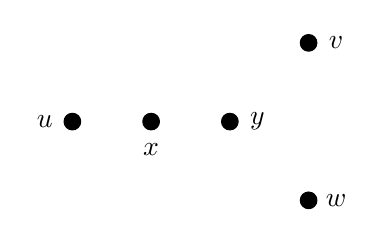
\begin{tikzpicture}
        \draw[fill=black] (0.0, 0.0) circle (3pt);
        \node at (-0.35, 0.0) {$u$};
        \draw[fill=black] (1.0, 0.0) circle (3pt);
        \node at (1.0, -.35) {$x$};
        \draw[fill=black] (2.0, 0.0) circle (3pt);
        \node at (2.35, 0.0) {$y$};
        \draw[fill=black] (3.0, 1.0) circle (3pt);
        \node at (3.35, 1.0) {$v$};
        \draw[fill=black] (3.0, -1.0) circle (3pt);
        \node at (3.35, -1.0) {$w$};
    \end{tikzpicture}

    $\downarrow$

    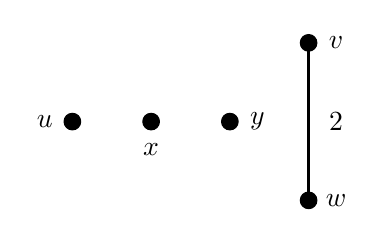
\begin{tikzpicture}
        \draw[fill=black] (0.0, 0.0) circle (3pt);
        \node at (-0.35, 0.0) {$u$};
        \draw[fill=black] (1.0, 0.0) circle (3pt);
        \node at (1.0, -.35) {$x$};
        \draw[fill=black] (2.0, 0.0) circle (3pt);
        \node at (2.35, 0.0) {$y$};
        \draw[fill=black] (3.0, 1.0) circle (3pt);
        \node at (3.35, 1.0) {$v$};
        \draw[fill=black] (3.0, -1.0) circle (3pt);
        \node at (3.35, -1.0) {$w$};

        \draw[thick] (3.0, -1.0) -- (3.0, 1.0);
        \node at (3.35, 0) {2};
    \end{tikzpicture}

    $\downarrow$

    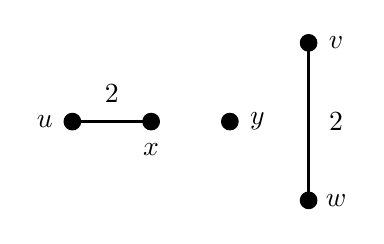
\begin{tikzpicture}
        \draw[fill=black] (0.0, 0.0) circle (3pt);
        \node at (-0.35, 0.0) {$u$};
        \draw[fill=black] (1.0, 0.0) circle (3pt);
        \node at (1.0, -.35) {$x$};
        \draw[fill=black] (2.0, 0.0) circle (3pt);
        \node at (2.35, 0.0) {$y$};
        \draw[fill=black] (3.0, 1.0) circle (3pt);
        \node at (3.35, 1.0) {$v$};
        \draw[fill=black] (3.0, -1.0) circle (3pt);
        \node at (3.35, -1.0) {$w$};

        \draw[thick] (3.0, -1.0) -- (3.0, 1.0);
        \node at (3.35, 0) {2};
        \draw[thick] (0,0) -- (1,0);
        \node at (.5,.35) {2};
    \end{tikzpicture}

    $\downarrow$

    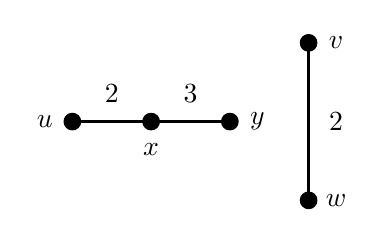
\begin{tikzpicture}
        \draw[fill=black] (0.0, 0.0) circle (3pt);
        \node at (-0.35, 0.0) {$u$};
        \draw[fill=black] (1.0, 0.0) circle (3pt);
        \node at (1.0, -.35) {$x$};
        \draw[fill=black] (2.0, 0.0) circle (3pt);
        \node at (2.35, 0.0) {$y$};
        \draw[fill=black] (3.0, 1.0) circle (3pt);
        \node at (3.35, 1.0) {$v$};
        \draw[fill=black] (3.0, -1.0) circle (3pt);
        \node at (3.35, -1.0) {$w$};

        \draw[thick] (3.0, -1.0) -- (3.0, 1.0);
        \node at (3.35, 0) {2};
        \draw[thick] (0,0) -- (1,0);
        \node at (.5,.35) {2};
        \draw[thick] (1.0,0) -- (2,0);
        \node at (1.5,.35) {3};
    \end{tikzpicture}

    $\downarrow$

    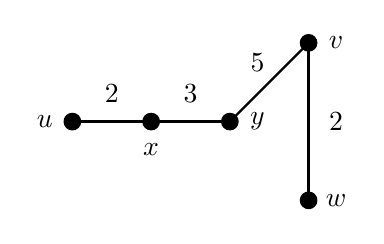
\begin{tikzpicture}
        \draw[fill=black] (0.0, 0.0) circle (3pt);
        \node at (-0.35, 0.0) {$u$};
        \draw[fill=black] (1.0, 0.0) circle (3pt);
        \node at (1.0, -.35) {$x$};
        \draw[fill=black] (2.0, 0.0) circle (3pt);
        \node at (2.35, 0.0) {$y$};
        \draw[fill=black] (3.0, 1.0) circle (3pt);
        \node at (3.35, 1.0) {$v$};
        \draw[fill=black] (3.0, -1.0) circle (3pt);
        \node at (3.35, -1.0) {$w$};

        \draw[thick] (3.0, -1.0) -- (3.0, 1.0);
        \node at (3.35, 0) {2};
        \draw[thick] (0,0) -- (1,0);
        \node at (.5,.35) {2};
        \draw[thick] (1.0,0) -- (2,0);
        \node at (1.5,.35) {3};
        \draw[thick] (2,0) -- (3,1);
        \node at (2.35, .75) {5};
    \end{tikzpicture}
\end{center}

\newpage
Prim's Algorithm:
\begin{center}
    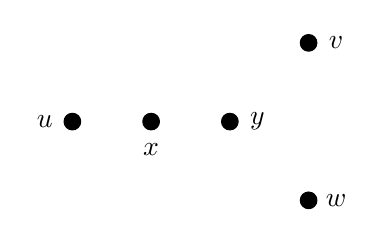
\begin{tikzpicture}
        \draw[fill=black] (0.0, 0.0) circle (3pt);
        \node at (-0.35, 0.0) {$u$};
        \draw[fill=black] (1.0, 0.0) circle (3pt);
        \node at (1.0, -.35) {$x$};
        \draw[fill=black] (2.0, 0.0) circle (3pt);
        \node at (2.35, 0.0) {$y$};
        \draw[fill=black] (3.0, 1.0) circle (3pt);
        \node at (3.35, 1.0) {$v$};
        \draw[fill=black] (3.0, -1.0) circle (3pt);
        \node at (3.35, -1.0) {$w$};

        % \draw[thick] (3.0, -1.0) -- (3.0, 1.0);
        % \node at (3.35, 0) {2};
        % \draw[thick] (0,0) -- (1,0);
        % \node at (.5,.35) {2};
        % \draw[thick] (1.0,0) -- (2,0);
        % \node at (1.5,.35) {3};
        % \draw[thick] (2,0) -- (3,1);
        % \node at (2.35, .75) {5};
    \end{tikzpicture}

    $\downarrow$

    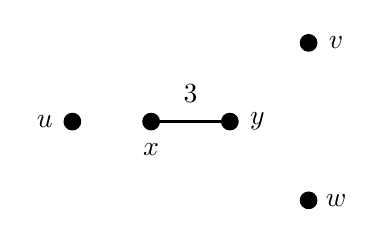
\begin{tikzpicture}
        \draw[fill=black] (0.0, 0.0) circle (3pt);
        \node at (-0.35, 0.0) {$u$};
        \draw[fill=black] (1.0, 0.0) circle (3pt);
        \node at (1.0, -.35) {$x$};
        \draw[fill=black] (2.0, 0.0) circle (3pt);
        \node at (2.35, 0.0) {$y$};
        \draw[fill=black] (3.0, 1.0) circle (3pt);
        \node at (3.35, 1.0) {$v$};
        \draw[fill=black] (3.0, -1.0) circle (3pt);
        \node at (3.35, -1.0) {$w$};

        % \draw[thick] (3.0, -1.0) -- (3.0, 1.0);
        % \node at (3.35, 0) {2};
        % \draw[thick] (0,0) -- (1,0);
        % \node at (.5,.35) {2};
        \draw[thick] (1.0,0) -- (2,0);
        \node at (1.5,.35) {3};
        % \draw[thick] (2,0) -- (3,1);
        % \node at (2.35, .75) {5};
    \end{tikzpicture}

    $\downarrow$

    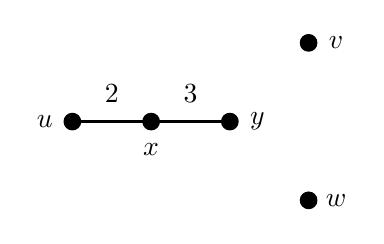
\begin{tikzpicture}
        \draw[fill=black] (0.0, 0.0) circle (3pt);
        \node at (-0.35, 0.0) {$u$};
        \draw[fill=black] (1.0, 0.0) circle (3pt);
        \node at (1.0, -.35) {$x$};
        \draw[fill=black] (2.0, 0.0) circle (3pt);
        \node at (2.35, 0.0) {$y$};
        \draw[fill=black] (3.0, 1.0) circle (3pt);
        \node at (3.35, 1.0) {$v$};
        \draw[fill=black] (3.0, -1.0) circle (3pt);
        \node at (3.35, -1.0) {$w$};

        % \draw[thick] (3.0, -1.0) -- (3.0, 1.0);
        % \node at (3.35, 0) {2};
        \draw[thick] (0,0) -- (1,0);
        \node at (.5,.35) {2};
        \draw[thick] (1.0,0) -- (2,0);
        \node at (1.5,.35) {3};
        % \draw[thick] (2,0) -- (3,1);
        % \node at (2.35, .75) {5};
    \end{tikzpicture}

    $\downarrow$

    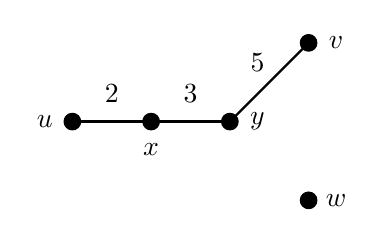
\begin{tikzpicture}
        \draw[fill=black] (0.0, 0.0) circle (3pt);
        \node at (-0.35, 0.0) {$u$};
        \draw[fill=black] (1.0, 0.0) circle (3pt);
        \node at (1.0, -.35) {$x$};
        \draw[fill=black] (2.0, 0.0) circle (3pt);
        \node at (2.35, 0.0) {$y$};
        \draw[fill=black] (3.0, 1.0) circle (3pt);
        \node at (3.35, 1.0) {$v$};
        \draw[fill=black] (3.0, -1.0) circle (3pt);
        \node at (3.35, -1.0) {$w$};

        % \draw[thick] (3.0, -1.0) -- (3.0, 1.0);
        % \node at (3.35, 0) {2};
        \draw[thick] (0,0) -- (1,0);
        \node at (.5,.35) {2};
        \draw[thick] (1.0,0) -- (2,0);
        \node at (1.5,.35) {3};
        \draw[thick] (2,0) -- (3,1);
        \node at (2.35, .75) {5};
    \end{tikzpicture}

    $\downarrow$

    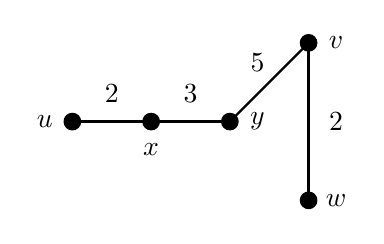
\begin{tikzpicture}
        \draw[fill=black] (0.0, 0.0) circle (3pt);
        \node at (-0.35, 0.0) {$u$};
        \draw[fill=black] (1.0, 0.0) circle (3pt);
        \node at (1.0, -.35) {$x$};
        \draw[fill=black] (2.0, 0.0) circle (3pt);
        \node at (2.35, 0.0) {$y$};
        \draw[fill=black] (3.0, 1.0) circle (3pt);
        \node at (3.35, 1.0) {$v$};
        \draw[fill=black] (3.0, -1.0) circle (3pt);
        \node at (3.35, -1.0) {$w$};

        \draw[thick] (3.0, -1.0) -- (3.0, 1.0);
        \node at (3.35, 0) {2};
        \draw[thick] (0,0) -- (1,0);
        \node at (.5,.35) {2};
        \draw[thick] (1.0,0) -- (2,0);
        \node at (1.5,.35) {3};
        \draw[thick] (2,0) -- (3,1);
        \node at (2.35, .75) {5};
    \end{tikzpicture}
\end{center}

\newpage\noindent{\bf ALSO}

\noindent{\bf 1.}

$S-e+f_1$:
\begin{center}
    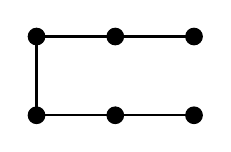
\begin{tikzpicture}
        \draw[fill=black] (0.0, 0.0) circle (3pt);
        \draw[fill=black] (1.0, 0.0) circle (3pt);
        \draw[fill=black] (2.0, 0.0) circle (3pt);
        \draw[fill=black] (0.0, 1.0) circle (3pt);
        \draw[fill=black] (1.0, 1.0) circle (3pt);
        \draw[fill=black] (2.0, 1.0) circle (3pt);

        \draw[thick] (0,0) -- (1,0);
        \draw[thick] (1,0) -- (2,0);
        \draw[thick] (2,1) -- (1,1);
        \draw[thick] (1,1) -- (0,1);
        \draw[thick] (0,1) -- (0,0); % f_1
    \end{tikzpicture}
\end{center}

$T+e-f_1:$
\begin{center}
    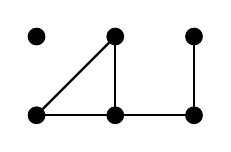
\begin{tikzpicture}
        \draw[fill=black] (0.0, 0.0) circle (3pt);
        \draw[fill=black] (1.0, 0.0) circle (3pt);
        \draw[fill=black] (2.0, 0.0) circle (3pt);
        \draw[fill=black] (0.0, 1.0) circle (3pt);
        \draw[fill=black] (1.0, 1.0) circle (3pt);
        \draw[fill=black] (2.0, 1.0) circle (3pt);

        \draw[thick] (0,0) -- (1,0);
        \draw[thick] (1,0) -- (2,0);
        \draw[thick] (2,0) -- (2,1); % f_3
        \draw[thick] (0,0) -- (1,1); % f_2
        \draw[thick] (1,1) -- (1,0); % e
    \end{tikzpicture}
\end{center}

$S-e+f_2:$
\begin{center}
    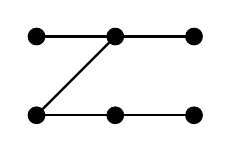
\begin{tikzpicture}
        \draw[fill=black] (0.0, 0.0) circle (3pt);
        \draw[fill=black] (1.0, 0.0) circle (3pt);
        \draw[fill=black] (2.0, 0.0) circle (3pt);
        \draw[fill=black] (0.0, 1.0) circle (3pt);
        \draw[fill=black] (1.0, 1.0) circle (3pt);
        \draw[fill=black] (2.0, 1.0) circle (3pt);

        \draw[thick] (0,0) -- (1,0);
        \draw[thick] (1,0) -- (2,0);
        \draw[thick] (2,1) -- (1,1);
        \draw[thick] (1,1) -- (0,1);
        \draw[thick] (0,0) -- (1,1); % f_2
    \end{tikzpicture}
\end{center}

$T+e-f_2:$
\begin{center}
    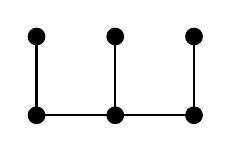
\begin{tikzpicture}
        \draw[fill=black] (0.0, 0.0) circle (3pt);
        \draw[fill=black] (1.0, 0.0) circle (3pt);
        \draw[fill=black] (2.0, 0.0) circle (3pt);
        \draw[fill=black] (0.0, 1.0) circle (3pt);
        \draw[fill=black] (1.0, 1.0) circle (3pt);
        \draw[fill=black] (2.0, 1.0) circle (3pt);

        \draw[thick] (0,0) -- (1,0);
        \draw[thick] (1,0) -- (2,0);
        \draw[thick] (2,0) -- (2,1); % f_3
        \draw[thick] (0,1) -- (0,0); % f_1
        \draw[thick] (1,1) -- (1,0); % e
    \end{tikzpicture}
\end{center}

$S-e+f_3:$
\begin{center}
    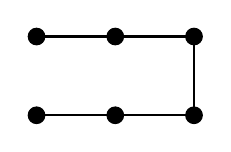
\begin{tikzpicture}
        \draw[fill=black] (0.0, 0.0) circle (3pt);
        \draw[fill=black] (1.0, 0.0) circle (3pt);
        \draw[fill=black] (2.0, 0.0) circle (3pt);
        \draw[fill=black] (0.0, 1.0) circle (3pt);
        \draw[fill=black] (1.0, 1.0) circle (3pt);
        \draw[fill=black] (2.0, 1.0) circle (3pt);

        \draw[thick] (0,0) -- (1,0);
        \draw[thick] (1,0) -- (2,0);
        \draw[thick] (2,1) -- (1,1);
        \draw[thick] (1,1) -- (0,1);
        \draw[thick] (2,0) -- (2,1); % f_3
    \end{tikzpicture}
\end{center}

$T+e-f_3:$
\begin{center}
    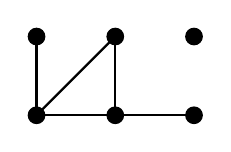
\begin{tikzpicture}
        \draw[fill=black] (0.0, 0.0) circle (3pt);
        \draw[fill=black] (1.0, 0.0) circle (3pt);
        \draw[fill=black] (2.0, 0.0) circle (3pt);
        \draw[fill=black] (0.0, 1.0) circle (3pt);
        \draw[fill=black] (1.0, 1.0) circle (3pt);
        \draw[fill=black] (2.0, 1.0) circle (3pt);

        \draw[thick] (0,0) -- (1,0);
        \draw[thick] (1,0) -- (2,0);
        \draw[thick] (0,1) -- (0,0); % f_1
        \draw[thick] (0,0) -- (1,1); % f_2
        \draw[thick] (1,1) -- (1,0); % e
    \end{tikzpicture}
\end{center}

\newpage\noindent{\bf 2.}

Lemma: If $T$ is a tree, then $T+uv$ contains exactly 1 cycle for all $u,v \in V(T)$ such that $uv \notin E(T)$.
\begin{proof}
    Let $T$ be a tree.
    Let $u,v \in V(T)$ such that $uv \notin E(T)$.
    
    Suppose that $T + uv$ contains the distinct cycles $A$ and $B$.
    Then, since $T$ is a tree, $uv$ is in both $A$ and $B$.
    Therefore, it is safe to assume that $A$ and $B$ are both of the form $(v, \hdots, u, v)$.\footnote{If they are not, simply rotate them until they are.}
    Let $P_A$ be the $v-u$ path obtained by removing the final entry from $A$.
    Let $P_B$ be the $v-u$ path obtained by removing the final entry from $B$.
    Note that $P_A \neq P_B$, since $A \neq B$.
    Let $P$ be the concatenation $P_A$ with the reverse of $P_B$.
    Since $P$ is a circuit, and $P$ does not contain $uv$, it must be that $T$ contains a cycle.
    Thus, $T$ is not a tree, so a contradiction has been demonstrated.
    Therefore, $T+uv$ contains less than 2 cycles.

    Since $u,v \in V(T)$, and $T$ is connected, there exists a $u-v$ path $P$ in $T$.
    Then, a cycle can be constructed by first following $P$, then following $vu$.
    Thus, $T$ contains exactly 1 cycle.
\end{proof}

Proposition: If $S$ and $T$ are spanning trees of a connected graph $G$, then for every edge $e \in E(S) \setminus E(T)$, there is an edge $f \in E(T) \setminus E(S)$ such that $S-e+f$ and $T+e-f$ are both spanning trees of $G$.
\begin{proof}
    Let $G$ be a connected graph.
    Let $S$ and $T$ be spanning trees of $G$.
    Let $e=uv \in E(S) \setminus E(T)$.

    Then, $S - e$ consists of two components, one containing $u$ and the other containing $v$.
    By Theorem 4.2, there is a unique $u-v$ path $P = (u, p_1, \hdots, v)$ in $T$.
    Thus, there exists an edge $f$ along $P$ that connects the components of $S - e$.
    Thus, $f$ is a bridge in $S - e + f$.
    Thus, since $S$ is a tree, every edge in $S-e+f$ is a bridge, so $S-e+f$ is a tree.
    Since $S-e+f$ is a tree with the same size and vertex set as $S$, and $S$ is a spanning tree of $G$, $S-e+f$ is therefore a spanning tree of $G$.

    Note that $P$ has length at least 2, since $e \notin E(T)$.
    Thus, $C = (u, p_1, \hdots, v, u)$ is a cycle in $T+e$.
    Then, by the lemma above, $C$ is the only cycle in $T+e$.
    Note that since $e \in E(S)$, $f \neq e$.
    Since removing $f$ from $T+e$ would eliminate $T+e$'s only cycle, $T+e-f$ thus has no cycles.
    Since $f$ lies on a cycle of $T+e$, $f$ is not a bridge in $T+e$, so $T+e-f$ is connected.
    Thus, $T+e-f$ is a tree.
    Since $T+e-f$ is a tree with the same size and vertex set as $S$, and $S$ is a spanning tree of $G$, $S+e-f$ is therefore a spanning tree of $G$.
\end{proof}

\newpage\noindent{\bf 4.30} Proposition: A connected weighted graph $G$ has a unique minimum spanning tree $T$ if and only if the weight of each edge $e$ of $G$ that is not in $T$ exceeds the weight of every other edge on the cycle in $T+e$.
\begin{proof}
    Let $G$ be a connected, weighted graph.

    Suppose that $G$ has a unique minimum spanning tree, $T$.
    Let $e \in E(G) \setminus E(T)$.
    By the lemma in the previous proof, $T+e$ contains exactly one cycle.
    Suppose $w(e) = w(f)$ for some edge $f \neq e$ along the cycle in $T+e$.
    Then, since $f$ lies along the cycle in $T+e$, it is not a bridge in $T+e$. % cite theorem
    Thus, $T+e-f$ is connected, and has no cycles.
    Thus, $T+e-f$ is a tree with $n-1$ edges and the same vertex set as $G$.
    Thus, since $w(e) = w(f)$, $T+e-f$ is a minimum spanning tree for $G$.
    Since $e \neq f$, $T+e-f \neq T$.
    Thus, $G$ does not have a unique minimum spanning tree, so it must be that $w(e) \neq w(f)$ for all $f \neq e$ along the cycle in $T+e$.

    We show the backward direction by contrapositive.
    Suppose that $T$ is not a unique minimum spanning tree of $G$.
    Then there exists another minimum spanning tree of $G$, $S$.
    By the result of the previous proof, there exist edges $e \in E(S) \setminus E(T), f \in E(T) \setminus E(S)$ such that $T - e + f$ and $S + e - f$ are both minimum spanning trees of $G$.
    Since all minimum spanning trees of $G$ must have the same weight, $w(e) = w(f)$.
    Thus, since $f \not\in E(T)$, there exists an edge not in $T$ which has a weight that does not exceed that of every edge in $T$.
\end{proof}

\newpage\noindent{\bf 5.2}

    {\bf (a)} For each integer $k \geq 2$, $K_{k,1}$ is a connected graph containing a vertex $v$ such that $G-v$ has $k$ components.
    This vertex is the only element of the order 1 partite set.

    {\bf (b)} $P_3$ is an example of such a graph.
    To see this, assign $u$ to be the vertex of degree 2, and $v$ to be either of the other vertices.

\newpage\noindent{\bf 5.4} Proposition: If $v$ is a cut-vertex of a graph $G$, then $v$ is not a cut-vertex of the complement $\overline{G}$ of $G$.

\begin{proof}
    Let $G$ be a graph, and let $v$ be a cut-vertex of $G$.
    Then, $G-v$ is disconnected.
    Thus, by Theorem 1.11, $\overline{G-v}$ is connected.
    Because neither graph contains $v$, $\overline{G-v} = \overline G - v$.
    Thus, $\overline G - v$ is connected.
    Thus, $v$ is not a cut vertex in $\overline G$.
\end{proof}

\newpage\noindent{\bf 5.6} Proposition: A $3$-regular graph $G$ has a cut-vertex if and only if $G$ has a bridge.

\begin{proof}
Let $G$ be a 3-regular graph.
Suppose that $G$ has a cut-vertex $u$.
Since $G$ is 3-regular, there exist exactly three vertices $\{v, w, x\} \subseteq V(G)$, adjacent to $u$.
These form the edges $uv, uw, ux \in E(G)$.

$\Longrightarrow$ Assume that $G$ has no bridges.
Consider the edge $uv$.
By Theorem 4.1, there $uv$ must belong to a cycle $C_{uv} = (u = v_0, v_1, \dots, v_k = v, u)$ in $G$.
Thus, the path $P_{uv} = (u = v_0, v_1, \dots, v_k = v)$ is present in $G - uv$.
Symmetric arguments show that there exist paths $P_{uw}$ and $P_{ux}$ such that $uw \notin P_{uw}$ and $ux \notin P_{ux}$.

Consider the graph $G - uv$.
Suppose that $uw$ is a bridge in $G-uv$. 
Then, by Theorem 4.1, $uw$ lies on no cycle in $G-uv$.
Thus, all cycles in $G$ containing $uw$ must also contain $uv$.
However, substituting $uv$ for $P_{uv}$ in $C_{uw}$, we obtain a cycle in $G-uv$ that contains $uw$.
This is a contradiction, so $uw$ is not a bridge in $G-uv$.
A symmetric argument shows that $ux$ is also not a bridge in $G-uv$.
Thus, in $G - uv - uw$, $ux$ must be a bridge since it is the only edge incident to $v$.
Thus, in $G - uv - uw - ux$, we have two components, one of which is $\{u\}$.
Thus, $G - uv - uw - ux - u$ has the same number of components as $G$.
This contradicts our assumption that $u$ is a cut-vertex in $G$, so it must be that $G$ contains a bridge.

$\Longleftarrow$ Now, assume that there is a bridge $e = uv \in E(G)$.
By definition, $\deg u = 3$.
By Theorem 5.1, $u$ is a cut-vertex in $G$.
\end{proof}

\newpage

\noindent\textbf{Exercise 5.8}
\begin{prop*}
Let $G$ be a nontrivial connected graph. If $v$ is an end-vertex of a spanning tree of $G$, then $v$ is not a cut-vertex of $G$.
\end{prop*}
\begin{proof}
Let $T$ be a spanning tree with $v$ as an end-vertex. Assume that $v$ is a cut-vertex of $G$. By Theorem 5.3/Corollary 5.4, there exist distinct $u,w \in V(G) \setminus \{v\}$ such that every u-w path contains $v$. Let such a path be $P = (u = w_0, w_1, \dots, v = w_i, \dots, v_k = v)$. Since an end-vertex of $T$ is a leaf, $\deg_T v = 1$. Thus, $v$ can only be an end-vertex of any subgraph of $T$. This implies that $P$ is not a subgraph of $T$ and so there is no path between $u$ and $w$ in $T$. Then $T$ is disconnected, which is a contradiction, so $v$ must not be a cut-vertex of $G$.
\end{proof}
\begin{prop*}
Every nontrivial connected graph contains at least two vertices that are not cut-vertices.
\end{prop*}
\begin{proof}
Any nontrivial connected graph has a spanning tree of order at least $2$. By Theorem 4.3, all such trees have at least two end-vertices. Thus by proved result (5a), every nontrivial connected graph has at least two vertices that are not cut-vertices.
\end{proof}
\begin{prop*}
Let $v$ be a vertex in a nontrivial connected graph $G$. There exists a spanning tree of $G$ that contains all edges of $G$ that are incident with $v$.
\end{prop*}
\begin{proof}
Let the order of $G$ be $n$ and its size be $m$. Since $G$ is an unweighted graph, let all edges in $G$ have the same weight. Now apply Kruskal's algorithm. First, let  $H_0$ be a subgraph of $G$ such that $V(H_0) = V(G)$ and $E(H_0) = \emptyset$. We know that $\deg_G v = k$, so $m \geq k$. Since all edges in $G$ have the same weight, we can add each edge incident to $v$ according to the algorithm, arriving at the spanning subgraph $H_k$. Now continue applying Kruskal's algorithm for the rest of the edges in $G$, resulting in the subgraph $H_{n-1}$. Note that by Theorem 4.7, $m \geq n-1$. By Theorem 4.11, this algorithm produces a spanning tree of $G$, which contains every edge incident to $v$ in $G$.
\end{proof}
\begin{prop*}
If a connected graph $G$ has exactly two vertices that are not cut-vertices, then $G$ is a path.
\end{prop*}
\begin{proof}
By Theorem 4.10, any connected graph has a spanning tree $T$. By assumption, $G$ has order $n \geq 2$, so by Theorem 4.3, $T$ has at least two leaves. Note that a tree with vertices of degree greater than two has more than two leaves. By proved result (5a), every end-vertex of $T$ is not a cut-vertex of $G$. Thus, all vertices in $G$ have degree $2$ or $1$.

Let $v \in V(G)$ such that $\deg_G v = 1$. Then any path that includes $v$ will be of the form
\[
P = (v = v_0, v_1, \dots, v_k).
\]
By Theorem 5.3/Corollary 5.4, $v$ is not a cut-vertex. Thus, there are exactly two vertices of degree $1$ in $G$.

Let $u,w \in V(G)$ be distinct vertices and let
\[
P = (u = w_0, w_1, \dots, w_k = w)
\]
be a path of maximum length in $G$. Suppose that $G$ is not a path. Then there exists some vertex $w \not\in P$ which is adjacent to some vertex in $P$.

\textbf{Case 1}: Let $x \in V(P)$ such that $\deg_P = 2$. Assume that $w$ is adjacent to $x$ in $G$. Then $\deg_G x = 3$. This is a contradiction.

\textbf{Case 2}: Let $y \in V(P)$ such that $\deg_P y = 1$. Assume that $w$ is adjacent to $y$ in $G$. Then we can append $w$ to $P$, creating a path with one more vertex than $P$. This contradicts our choice of $P$.

Thus, $G = P$.
\end{proof}

\end{document}